\chapter{Resultater}

I denne del af rapporten fremlægges projektets resultater fra modultesten, integrationstesten og  accepttesten. Der fokuseres på kun få udvalgt resultater, der er vigtige for produktets funktionsdygtighed,  fra hver af de nævnte testtyper. De fulde resultater, der er opnåede under disse tests henvises der til de pågældende bilag. I det følgende præsenteres første hardware resultaterne, der er opnåede i modultesten og integrationstesten efterfulgt af software resultaterne, der opnåede inden for det samme testtype. Tilslut fremvises accepttestens resultater.     

\section{Modultest}
\subsection{Hardware}
Under modultesten af hardwaredelen er der opnåede resultater for hver af de testede moduler, se disse resultater i \nameref{bilag6}. En af de kritiske opnåede resultater for hele systemet var resultatet fra strømgeneratoren. Figur \ref{fig:Stromgeneratorload} viser strømproduktion af strømgeneratoren. Her ses at strømmen er konstant, når belastningen varieres op til $10k \Omega$, hvilken er den højeste impedans som et menneskevæv kan levere\cite[s. 49]{Chester2014}. Til at skabe en ohmsk ændring, er der anvendt en variabel modstand.        

\begin{figure}[H] 
\centering
{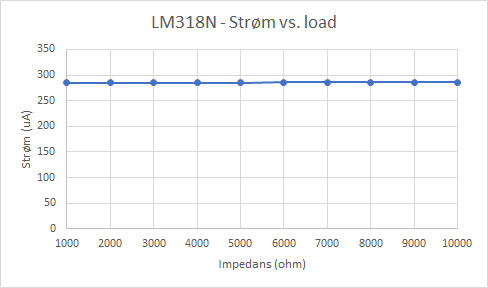
\includegraphics[width=12cm]
{Figure/Stromgeneratorload}}
\caption{Output-strømmen af strømgeneratoren, når belastningen varieres fra $1 - 10k\Omega$}
\label{fig:Stromgeneratorload}
\end{figure}


\pagebreak 

Et andet vigtigt resultatet for hele systemet var resultatet af systemets AA filter. For at afgøre, hvor meget filterets dæmpning skal være, sammensættes alle systemets komponenter for at lave en spektrumanalyse. På \ref{fig:aaspectrum1} kan man aflæse amplituden på den målte signal, samt hvor meget amplituden er dæmpet ved 250 kHz, som er den halve samplingfrekvens. Det kan aflæses at signalet er aftaget med 75dB. Dette betyder at systemets AA-filter skal dæmpe signalet yderligere med 15 dB  for at opfylde ADC'ens bit range, som er 90 dB.   

       
\begin{figure}[H] 
\centering
{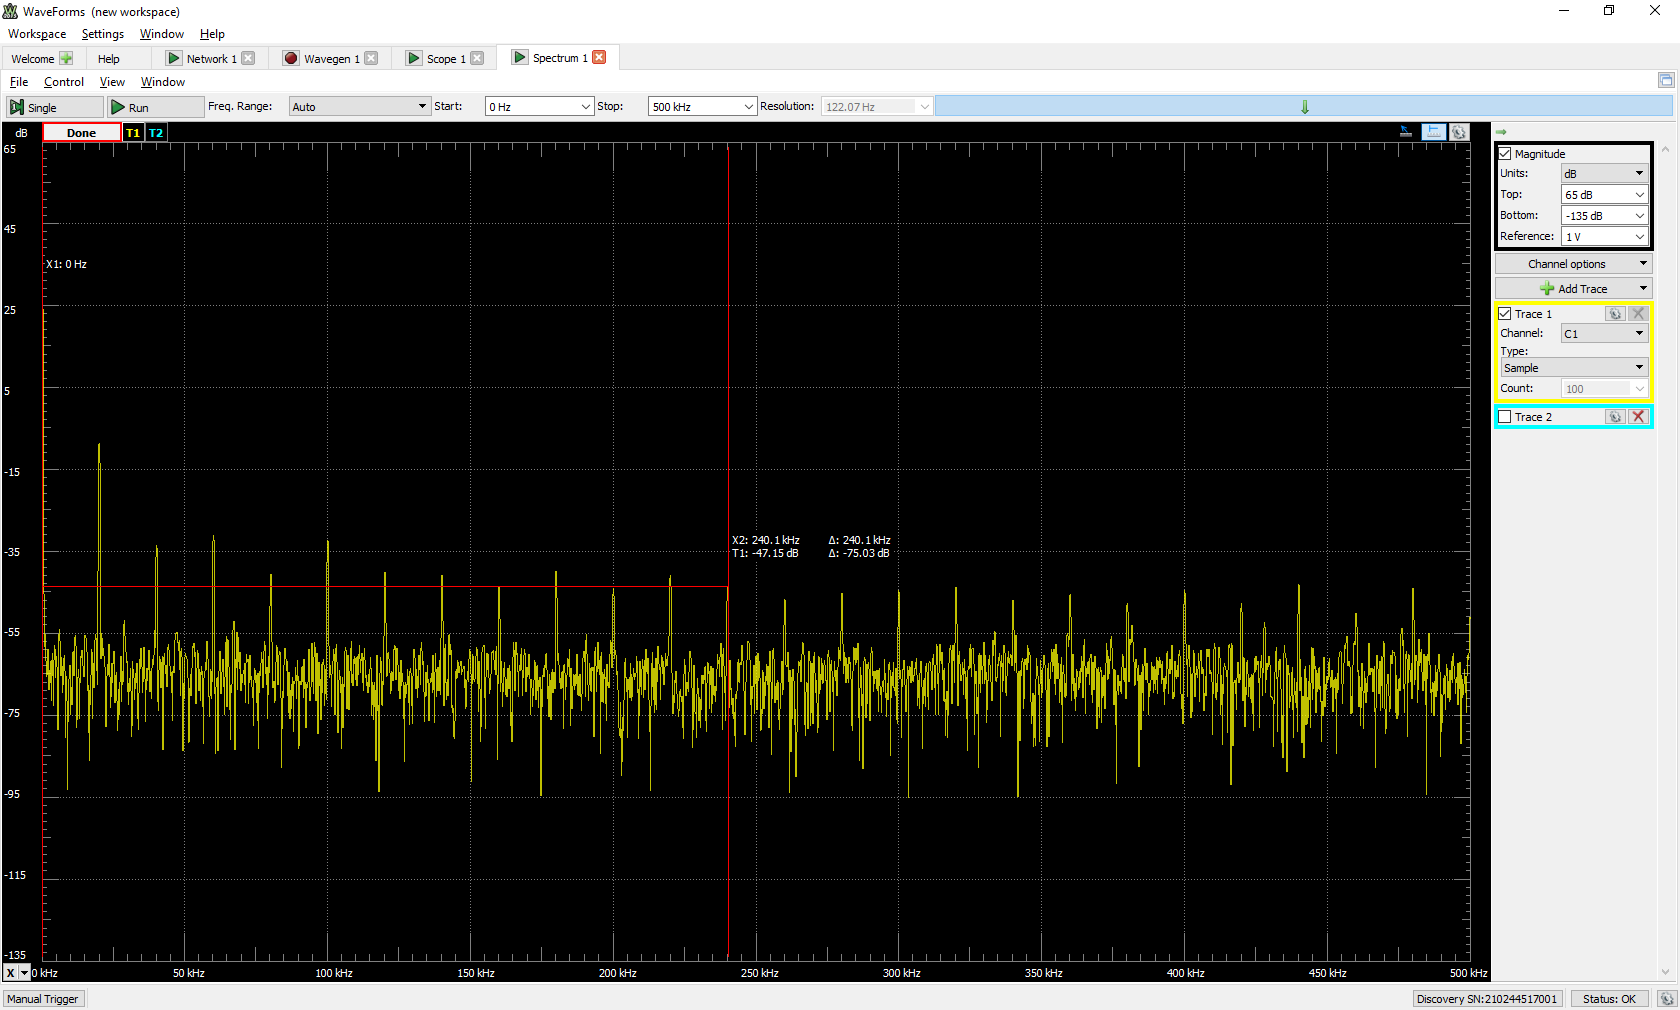
\includegraphics[width=\linewidth]
{Figure/aaspectrum1}}
\caption{Det implementeret frekvensspektrum, som viser at der er en samlet dæmpning på ca. 75dB som skal yderligere dæmpes til 90dB med et 2.ordens lavpasfilter.}
\label{fig:aaspectrum1}
\end{figure}

\pagebreak

Da man nu kender, hvor meget signalet skal dæmpes, designes der et 2. ordens lavpasfilter. På figur \ref{fig:aafiltermodultest} ses at filteret er i stand til at dæmpe et signal med mere end 15dB. 


\begin{figure}[H] 
\centering
{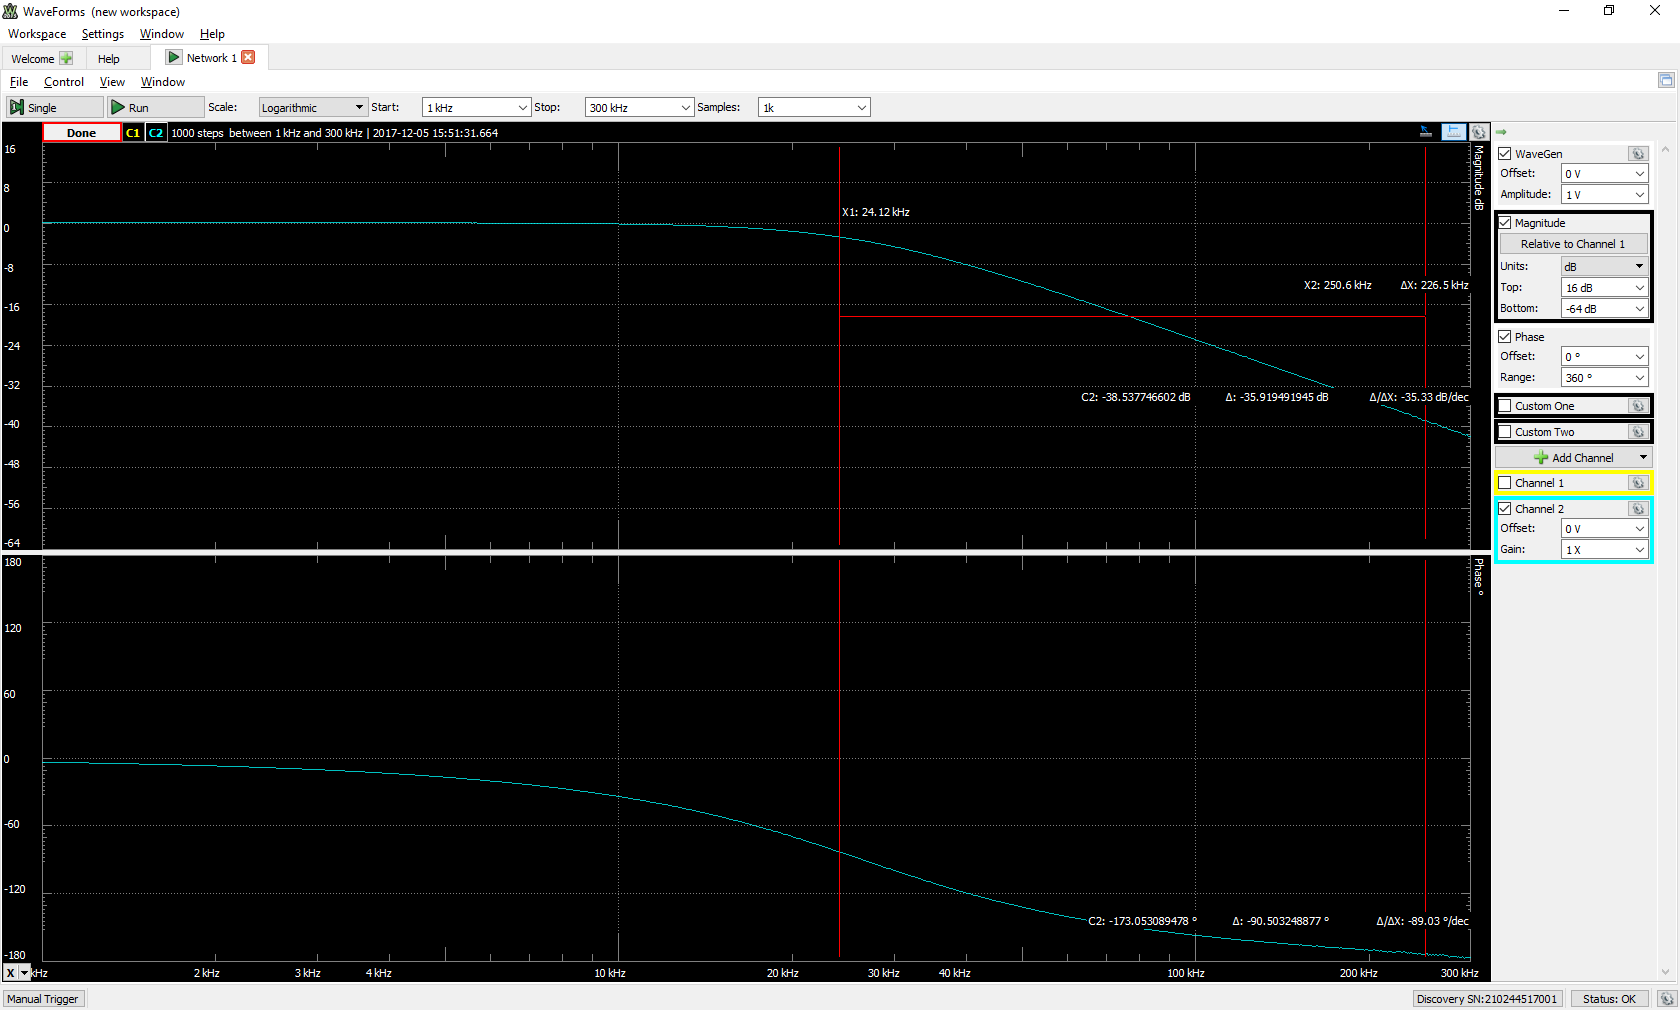
\includegraphics[width=\linewidth]
{Figure/aafiltermodultest}}
\caption{Resultat om filterets virkning fra Network Analyzer i waveforms.}
\label{fig:aafiltermodultest}
\end{figure}




\subsection{Software}

Under modultesten af softwaredelen er der opnåede resultater for hver af de testede moduler, se disse resultater i \nameref{bilag6}. En af de kritiske opnåede resultater for hele systemet var resultatet fra funktionen \textit{"Read\_Measurements"}. Dette resultat kan ses på figur \ref{fig:modultestshow}. Resultatet viser den ønskede simultane måling af to signaler. 

\begin{figure}[H] 
\centering
{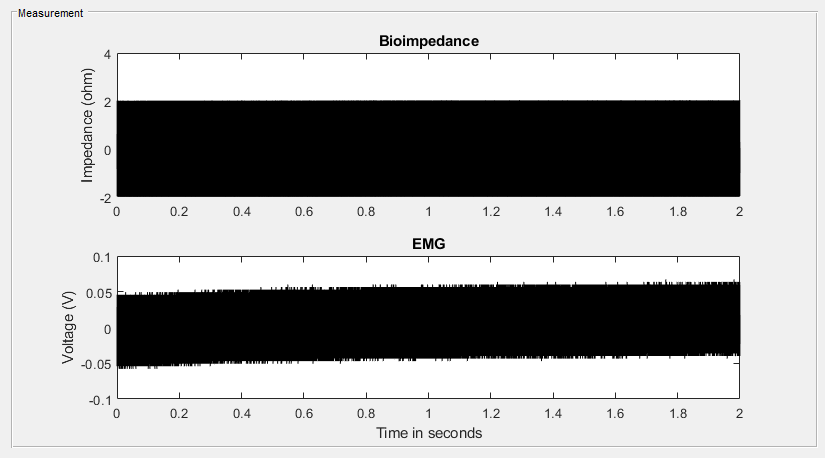
\includegraphics[width=10cm]
{Figure/modultestshow}}
\caption{Den ønskede simultane måling med to signaler.}
\label{fig:modultestshow}
\end{figure}


I funktionen Process\_Measurements blev bl.a. Bi signalet behandlet ved brug af envelope. Dette resulterede først i at BI signalet blev dobbelt ensrettet, hvilket kan ses i figur \ref{fig:modultestprocessEnsrettet}. Ved at se på det oprindelige BI signal (rød), går det over til at blive dobbelt ensrettet (blå). 

\begin{figure}[H] 
\centering
{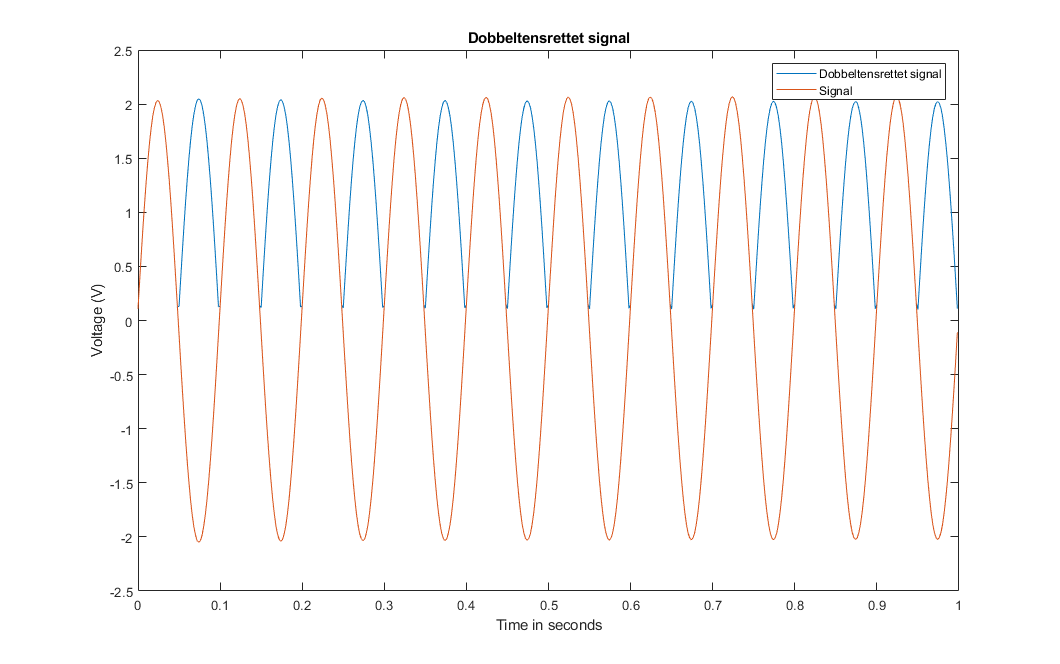
\includegraphics[width=10cm]
{Figure/modultestprocessEnsrettet}}
\caption{Resultatet af dobbelt ensretning af BI signalet.}
\label{fig:modultestprocessEnsrettet}
\end{figure}

Dernæst blev BI signalet lavpas filteret, se figur \ref{fig:modultestprocessFilter}.

\begin{figure}[H] 
\centering
{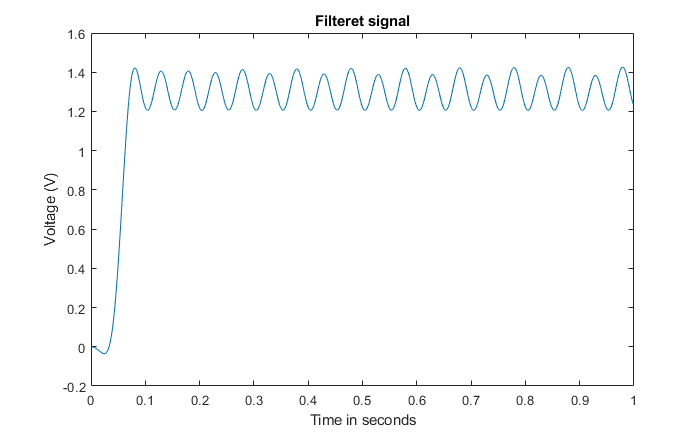
\includegraphics[width=10cm]
{Figure/modultestprocessFilter}}
\caption{Resultatet efter BI signalet er blevet lavpas filteret}
\label{fig:modultestprocessFilter}
\end{figure}


\section{Integrationstest}

I integrationstesten, bliver alle modulerne samlet til et system. Dette blev gjort vha. Top-down metoden hvor hver enkelt modul løbende blev tilføjet. Undervejs blev der noteret spændinger og ændringer for hvert modul. Dette resulterede i tabel \ref{tab:inout}. 

\begin{table}[H]
\center
\begin{tabularx}{\linewidth}{l  X  X}
     \textbf{Navn}	&	\textbf{Input}		&	\textbf{Output}  \\ \midrule
     
     Analog Discovery	&		&	2 V / 20 kHz         \\   \addlinespace[2mm]
     Instrumentationsforstærker 1	&	2 V / 20 kHz	&	4 V / 20 kHz         \\   \addlinespace[2mm]
     VCCS	&	4 V / 20 kHz	&	283 uA / 20 kHz        \\   \addlinespace[2mm]
     Instrumentationsforstærker 2	&	Biosignal	&	1,67 V         \\   \addlinespace[2mm]
     Op-AMP	&	1,67 V 	&	14,3 V        \\   \addlinespace[2mm]	
     AA filter	&	14,3 V 	&	13,4 V        \\   \addlinespace[2mm]
     \bottomrule                                                                                                                   
    \end{tabularx}
    \caption {Oversigt over input og output for hver komponent..}
    \label{tab:inout}
	
\end{table}

Da elektroderne blev påsat måleobjektet, kunne det konstateres at den stabile strøm på 283 $\mu A$ se figur \ref{fig:integrationstestVCCSud} ændrede sig til 104 $\mu A$ se figur \ref{fig:integrationstestINA2udstrom}.

\begin{figure}[H]
\centering
\begin{minipage}{.5\textwidth}
  \centering
  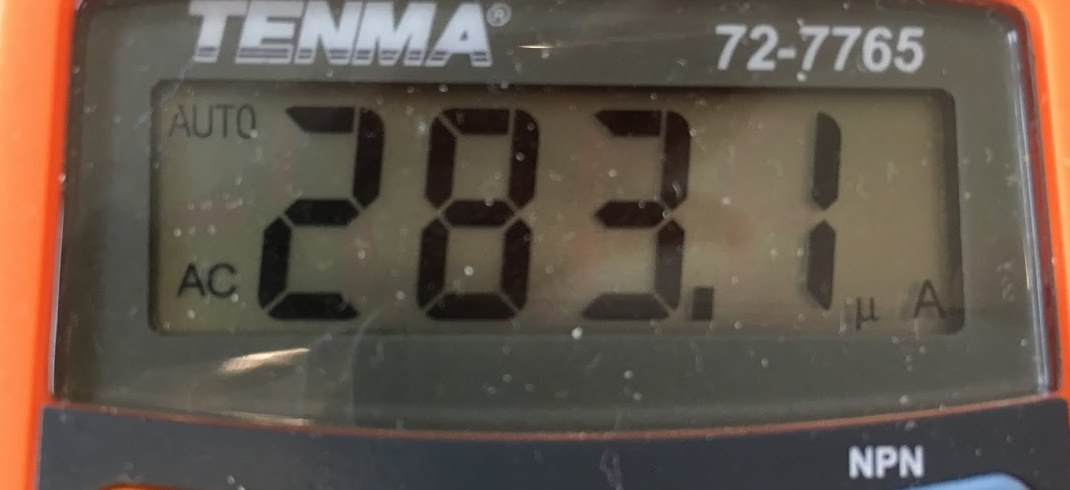
\includegraphics[width=.6\linewidth]{Figure/integrationstestVCCSud}
  \captionof{figure}{Strømmen uden påsatte elektroder}
  \label{fig:integrationstestVCCSud}
\end{minipage}%
\begin{minipage}{.5\textwidth}
  \centering
  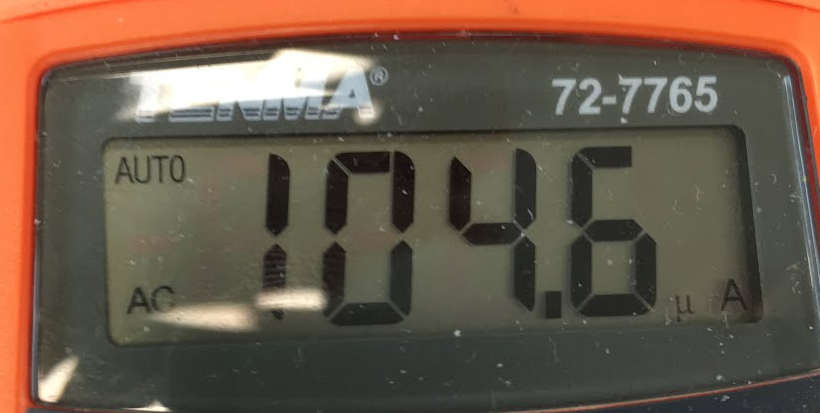
\includegraphics[width=.6\linewidth]{Figure/integrationstestINA2udstrom}
  \captionof{figure}{Strømmen med påsatte elektroder}
  \label{fig:integrationstestINA2udstrom}
\end{minipage}
\end{figure}

Efter AA filter er blevet tilføjet var det muligt at lave en ny spektrum analyse. Dette resultat kan ses på figur \ref{fig:integrationstestAAspectrum}. AA filter's dæmping kunne nu aflæses til 95 dB ved 250 kHz.

\begin{figure}[H] 
\centering
{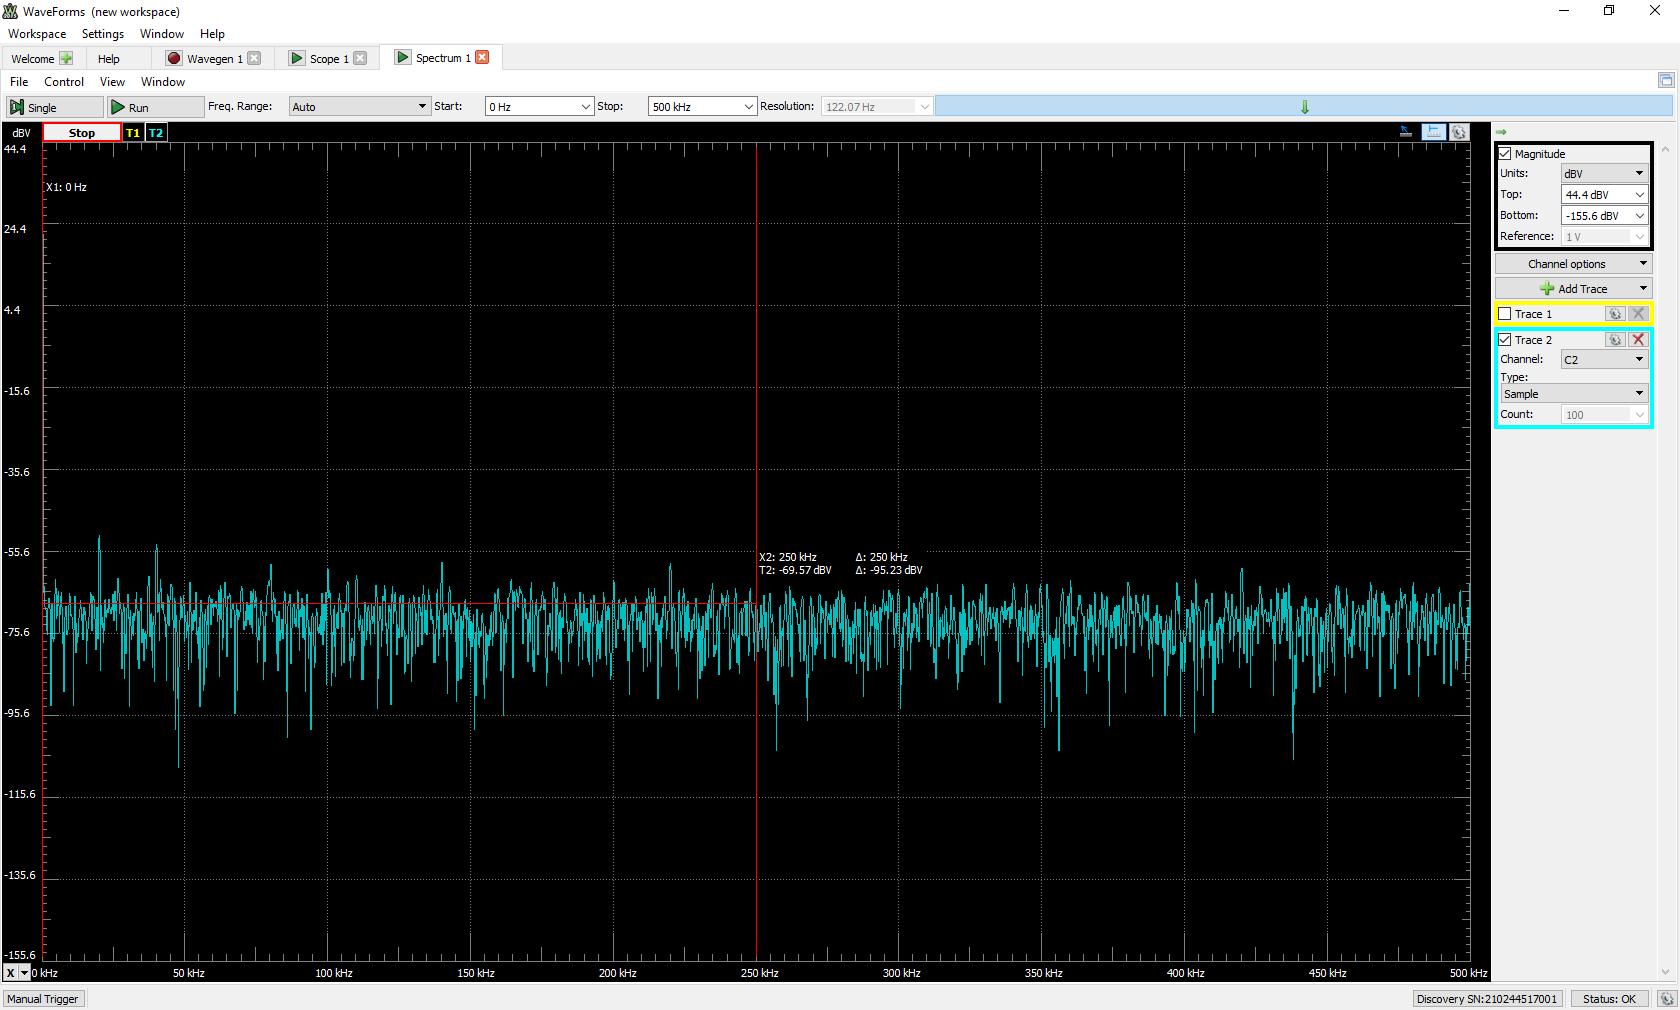
\includegraphics[width=\linewidth]
{Figure/integrationstestAAspectrum}}
\caption{Resultatet af den nye spektrumanalyse.}
\label{fig:integrationstestAAspectrum}
\end{figure}


Da MyoWare Muscle Sensor blev tilføjet, aflæses den konstante strøm til at være 283 $\mu A$, se figur \ref{fig:integrationstestVCCSud2}.

 
%\begin{figure}[H] 
%\centering
%{\includegraphics[width=4cm]
%{Figure/myoware}}
%\caption{MyoWare Muscle Sensor }
%\label{fig:myoware}
%\end{figure}

\begin{figure}[H] 
\centering
{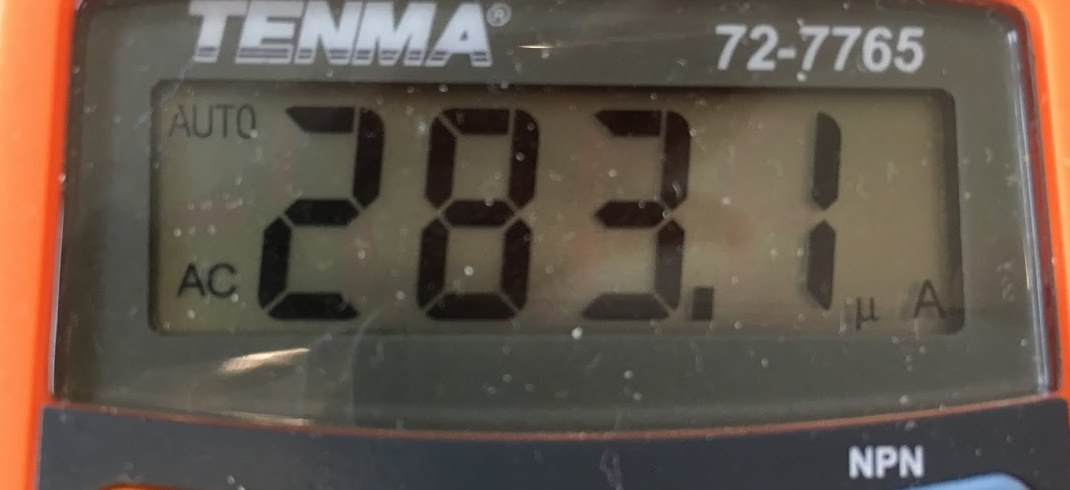
\includegraphics[width=6cm]
{Figure/integrationstestVCCSud}}
\caption{Resultatet efter BI signalet er blevet lavpas filteret}
\label{fig:integrationstestVCCSud2}
\end{figure}

Figur \ref{fig:guiDone} viser resultatet af den sidste del af integrationstesten. Resultatet viser et målt BI signal og EMG signal simultant. Det kan også ses at hvert synk i BI signalet har samtidig udslag i EMG målingen. Det kan også ses at antal synk bliver registeret og vist. 

\begin{figure}[H] 
\centering
{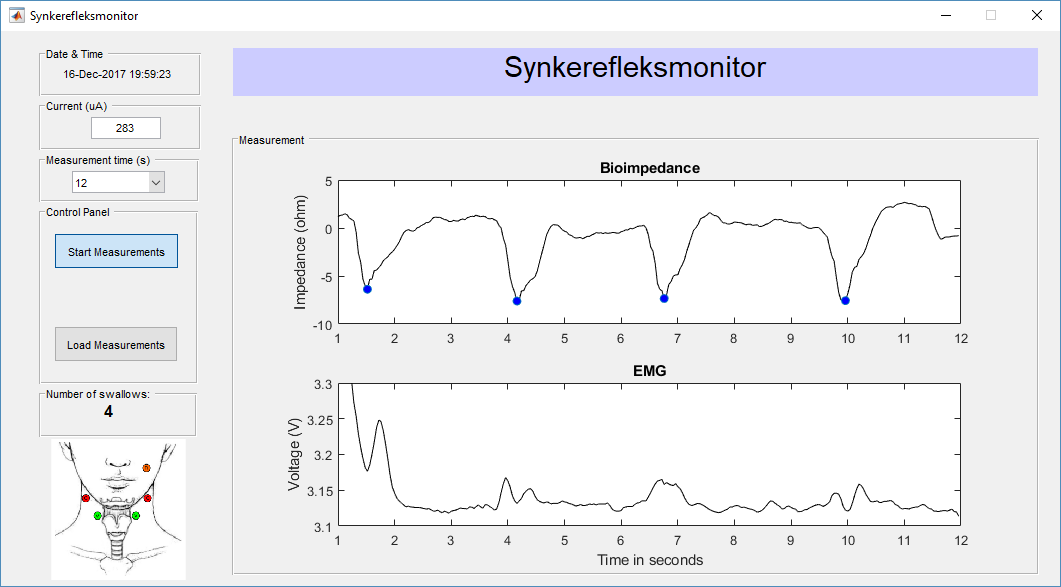
\includegraphics[width=\linewidth]
{Figure/guiDone}}
\caption{Resultatet af integrationen af hardware og software.}
\label{fig:guiDone}
\end{figure}



\section{Accepttest}
\subsection{Funktionelle krav}
De funktionelle krav som dette projekt har prioriteret højst er de krav, der er defineret i \textit{Must og Should}. Til opfyldelsen af disse krav, er der benyttet use cases, der sammen definerer, hvordan disse krav opnås. De detaljeret testudførsel og resultater kan læses i \nameref{bilag6}. I tabel \ref{AT_UC1} præsenteres use casens resultat udfald. 
  
\begin{longtabu} to \linewidth{@{} c X[l] X[l] X[j] c@{}}
    ~ &	\textbf{Use case nr.} &    \textbf{Krav type} &		\textbf{Testresultat} \\[-1ex]
    \midrule
    ~ & 1 & Funktionelle krav & Godkendt &
    \\ \midrule
   &   2 &   Funktionelle krav & Godkendt   &	
   
\\ \midrule
   &   3 &   Funktionelle krav & Godkendt   &   
   
 \\ \bottomrule
 
\caption{Resultaterne for de funktionelle krav, der er defineret i kravspecifikationen}\\
\label{AT_UC1}
\end{longtabu}


De tre use cases tilsammen opfylder kravene i \textit{Must og Should} i kravspecifikationen med undtagelse krav nummer 9. Se kapitel 7, hvorfor dette krav ikke er opfyldt. 

\pagebreak
\subsection{Ikke-funktionelle krav}

Tilforskel fra de funktionelle krav er de ikke-funktionelle krav ikke organiseret i use cases. De ikke-funktionelle krav består af punkter, der definerer produktets kvalitetsaspekter. Disse skal være testbart. Herunder opsummeres resultaterne af accepttesen for de ikke-funktionelle krav. 

\begin{longtabu} to \linewidth{@{} c X[l] X[l] X[j] c@{}}
    ~ &	\textbf{Krav nr.} &    \textbf{Krav type} &		\textbf{Testresultat} \\[-1ex]
    \midrule
    ~ & 1 & ikke-funktionelle krav & ej testbart &
    \\ \midrule
   &   2 &   ikke-funktionelle krav & ej testbart   &	
   
\\ \midrule
   &   3 &   ikke-funktionelle krav & ej testbart   &   
   
   \\ \midrule
   &   4 &   ikke-funktionelle krav & Godkendt   &  
   
   
    \\ \midrule
   &   5 &   ikke-funktionelle krav & Godkendt   & 
   
    \\ \midrule
   &   6 &   ikke-funktionelle krav &  ej testbart  & 
   
   
    \\ \midrule
   &   7 &   ikke-funktionelle krav &  ej testbart  & 
     \\ \midrule
   &   8 &   ikke-funktionelle krav & Godkendt  & 
     \\ \midrule
   &   9 &   ikke-funktionelle krav &  ej testbart  &  
   \\ \midrule
    &   10 &   ikke-funktionelle krav &  Godkendt  &  
    
    \\ \midrule
    &   11 &   ikke-funktionelle krav &  Godkendt  &  
   
   
 \\ \bottomrule
 
\caption{Resultaterne for de ikke-funktionelle krav, der er defineret i kravspecifikationen}\\
\label{AT_UC2}
\end{longtabu}

Som det ses i tabel \ref{AT_UC2} er der en del krav, der er mærkeret som ej testbart under accepttesten. Gruppen har været fuld bevidst om at disse krav ikke er testbart, men har alligevel medtaget som et ønsket kvalitets parametre. Dette valg er truffet for at gøre brugeren/kunden opmærksom på, at produktet ikke er testet under de nævnte forhold og dermed skal brugeren være opmærksom på at anvende produktet under disse forhold, der ikke testet.  